62. $y=\cfrac{3x^2+8x+4}{|2x+2|+x}=\cfrac{(3x+2)(x+2)}{|2x+2|+x}=\begin{cases} \cfrac{(3x+2)(x+2)}{3x+2}=x+2,\ x\geqslant-1,\ x
eq-\cfrac{2}{3},\\ \cfrac{(3x+2)(x+2)}{-x-2}=-3x-2,\ x<-1,\ x
eq-2.\end{cases}$
$$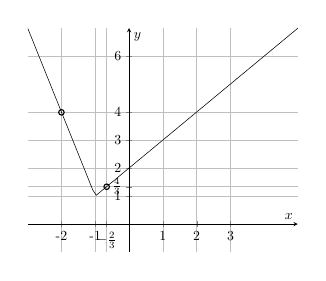
\begin{tikzpicture}[scale=0.5]
\begin{axis}[
    axis lines = middle,
    grid=major,
    legend pos={south west},
    xlabel = {$x$},
    ylabel = {$y$},
    ymin=-1,
    ymax=7,
    xtick={-3,-1,1,3,5,2,-2,-0.666},
    xticklabels={-3,-1,1,3,5,2,-2,$-\frac{2}{3}$},
    ytick={ 6, 2,-6, -2,1,4,-4,3,-3,1.333},
    yticklabels={ 6, 2,-6, -2,1,4,-4,3,-3,$\frac{4}{3}$}           ]
	\addplot[domain=-4:6, samples=100, color=black] {(3*x*x+8*x+4)/(abs(2*x+2)+x)};
%\addplot[domain=-4:1, samples=100, color=black] {2-x};
%\addplot[domain=-3.1:2.5, samples=100, color=red] {70*abs(1-2*abs(abs(x)-2))-10*x^2+10*x-70};
	%\addlegendentry{$\text{Рис. 1}$};
\end{axis}
\draw (2,1.66) circle (2pt);
\draw (0.85,3.55) circle (2pt);
\end{tikzpicture}$$
По графику определим, что прямая $y=a$ не имеет с графиком общих точек при $a<1.$\\
